\scanpage{2}
\deleted{clearly \unsure{distinguish|determined} $\bar D_{J,\alpha}$ from $\bar D_J$, cf. \unsure{9}}
\deleted{\diagram{\begin{tikzcd}
\bar U_{J',\alpha'} \arrow[r] \arrow[d] & \bar U_{J,\alpha} \arrow[r] \arrow[d] & \bar U \arrow[d] \\
U_{J',\alpha'} \arrow[r] & U_{J,\alpha} \arrow[r] & U
\end{tikzcd}}}

\diagram{\begin{tikzcd}[column sep=small]
D=U(\mathbb C)^{\sim} \arrow[rr] \arrow[dr,"\pi"'] && \widetilde U(\mathbb C)\deleted{\unsure{\ne U|=U}} \arrow[dl,"\hat\pi"] \\
& U(\mathbb C) &
\end{tikzcd}}
\[ \pi\subset G \]
\[
H_{\deleted{\unsure{u}}}=\bigl\{u\in G\mid \exists
\underset{\substack{\text{\unsure{subgroup|subgroup}}\\\text{of finite index}}}{\begin{gathered}\pi'\subset\pi\\[-.8ex]
\begin{tikzpicture}[x=1cm,y=1cm,baseline=0pt]\draw (0,.09) .. controls (-.04,-.01) and (-.01,-.05) .. (.10,-.05)--(1.25,-.05) .. controls (1.38,-.05) and (1.38,.03) .. (1.30,.09);\end{tikzpicture}\end{gathered}},\quad
\underset{\text{ditto}}{\begin{gathered}\pi''\subset\pi\\[-.8ex]
\begin{tikzpicture}[x=1cm,y=1cm,baseline=0pt]\draw (0,.09) .. controls (-.04,-.01) and (-.01,-.05) .. (.10,-.05)--(1.25,-.05) .. controls (1.38,-.05) and (1.38,.03) .. (1.30,.09);\end{tikzpicture}\end{gathered}},
\quad\text{isomorphism }v:D/\pi'\simeq D/\pi'',\quad\text{with}
\]
\diagram{\begin{tikzcd}
D \arrow[r,"u"] \arrow[d,"p'"'] & D \arrow[d,"p''"] & \text{commutative} \\
D/\pi' \arrow[r,"\substack{v\\\sim}"] & D/\pi'' &
\end{tikzcd}}

\uline{NB} We shall have, for $u,\pi',\pi'',v$ as above an isomorphism
\figure{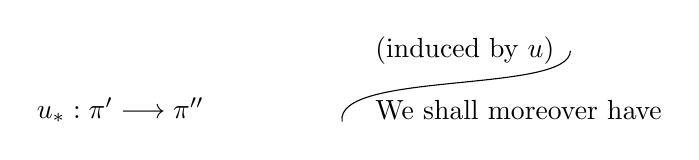
\begin{tikzpicture}
\node[anchor=west] (map) at (0,0) {$u_*:\pi'\longrightarrow\pi''$};
\node[anchor=west] (ins) at (4.3,.75) {\inserted{(induced by $u$)}};
\draw ([xshift=.08cm]ins.east) .. controls (6.9,.2) and (3.9,.5) .. (4,-.15);
\node[anchor=west] at (4.3,0) {We shall moreover have};
\end{tikzpicture}}
$\pi'$ and $\pi''$ of the same index in $\pi$.
\margin{$u$ is determined by $v_*$}

\uline{NB} $v$ is known when one knows $v_*$ (\uline{these conditions}), and when $v$ is known, $u$ is known \deleted{\unsure{to the}} modulo multiplication \uline{\unsure{on the|:} left} by a $\gamma\unsure{\in|+}\pi''$.

\margin{\diagram{\begin{tikzcd}[column sep=small]
& \pi & \\
\pi' \arrow[ur,phantom,"\tikz[baseline=-.5ex]{\node[rotate=-35,inner sep=0pt] {$\cup$};}" description] \arrow[rr,phantom,"\simeq" description] && \pi'' \arrow[ul,phantom,"\tikz[baseline=-.5ex]{\node[rotate=15,inner sep=0pt] {$\cup$};}" description]
\end{tikzcd}}
\[\pi_i'\simeq\pi_i''\]}
\margin{\[
p''u=vp'
\]
\[\deleted{p''u\gamma=}\]
\[p''(\gamma u)=(p''\gamma)u=p''u=vp')\]
\[\deleted{\pi\subset H}\]}

$H$ is a group $\supset\pi$, and $H/\pi$ (cosets \unsure{on the|:} right) is identified with a subset of \unsure{the set|one} of the ``germs'' \uline{of isomorphisms} \deleted{\unsure{of the}} $H$-groups of \unsure{finite|finite} index of $\pi$ of the same index

$H_n=$ subset of $H$ formed of the $u$ for which one can take $\pi',\pi''$ of index $n$.

$H_n$ is a \uline{subgroup}, and $\pi$ of index
\mspage{1}
